% ============================================================================
% Municipality-Scale Flood Risk Mapping in Magdalena, Colombia
% Using Sentinel-1 SAR and Ensemble Machine Learning (2015--2025)
% Authors: Cristian Espinal Maya, Santiago Jimenez Londono
% Format: arXiv preprint
% ============================================================================

\documentclass{article}

\usepackage{arxiv}

\usepackage[utf8]{inputenc}
\usepackage[T1]{fontenc}
\usepackage{hyperref}
\usepackage{url}
\usepackage{booktabs}
\usepackage{amsfonts}
\usepackage{amssymb}
\usepackage{amsmath}
\usepackage{nicefrac}
\usepackage{microtype}
\usepackage{graphicx}
\usepackage{multirow}
\usepackage{siunitx}
\sisetup{
    group-separator = {,},
    group-minimum-digits = 4,
}
\usepackage{natbib}
\usepackage{tabularx}
\usepackage{textcomp}

\graphicspath{{./figures/}}

\title{Municipality-Scale Flood Risk Mapping in Magdalena, Colombia, Using Sentinel-1 SAR and Ensemble Machine Learning (2015--2025)}

\author{
  Cristian Espinal Maya\thanks{Correspondence: cespinalm@eafit.edu.co. ORCID: \href{https://orcid.org/0009-0000-1009-8388}{0009-0000-1009-8388}} \\
  School of Applied Sciences and Engineering\\
  Universidad EAFIT\\
  Medell\'in, Colombia \\
  \texttt{cespinalm@eafit.edu.co} \\
  \And
  Santiago Jim\'enez Londo\~no\thanks{ORCID: \href{https://orcid.org/0009-0007-9862-7133}{0009-0007-9862-7133}} \\
  School of Applied Sciences and Engineering\\
  Universidad EAFIT\\
  Medell\'in, Colombia \\
  \texttt{sjimenez@eafit.edu.co} \\
}

\begin{document}
\maketitle

\begin{abstract}
A persistent scale mismatch limits the utility of satellite-based flood products for local governance: most operate at national resolution, while flood risk decisions in decentralized countries are made at the municipal level. We present a reproducible, open-access framework that delivers municipality-level flood risk statistics for all 30 municipalities of the Department of Magdalena, Colombia (\SI{23188}{\kilo\metre\squared}; $\sim$1.3 million inhabitants). The department encompasses diverse terrain ranging from the Sierra Nevada de Santa Marta (\SI{5775}{\metre} a.s.l.)---the world's highest coastal mountain range---to the Caribbean coastal lowlands, the Ci\'enaga Grande de Santa Marta (a Ramsar wetland), and the R\'io Magdalena floodplain. We processed Sentinel-1 C-band SAR scenes (2015--2025) within Google Earth Engine using adaptive Otsu thresholding to produce monthly water extent maps at \SI{10}{\metre} resolution, employing both ascending and descending orbit passes to mitigate radar shadow effects from the Sierra Nevada. Eighteen predictor variables spanning topographic, hydrological, climatic, land cover, and demographic domains were integrated into a weighted ensemble of Random Forest, XGBoost, and LightGBM, evaluated under spatial five-fold cross-validation. HAND, SAR flood frequency, and elevation were identified as dominant predictors via SHAP analysis. Overlaying the susceptibility surface with \SI{100}{\metre} population data quantifies the population residing in high or very high susceptibility zones. La Ni\~na years amplify mean flood extent relative to El Ni\~no years. The entire framework---data, code, and trained models---is open-access and fully reproducible using Google Earth Engine and publicly available scripts (\url{https://github.com/Cespial/magdalena_flood_risk_research}), enabling direct replication across other tropical departments.
\end{abstract}

\keywords{flood susceptibility mapping \and Sentinel-1 SAR \and ensemble machine learning \and HAND \and Google Earth Engine \and SHAP \and ENSO \and population exposure \and Magdalena Colombia}

%%%%%%%%%%%%%%%%%%%%%%%%%%%%%%%%%%%%%%%%%%
\section{Introduction}
\label{sec:introduction}

Between November 2010 and May 2011, a La Ni\~na event struck Colombia with exceptional intensity: over 300 people died, 2.3 million were displaced, and direct losses exceeded USD 7.8 billion \citep{Hoyos2013}. The Department of Magdalena was among the hardest-hit regions---the R\'io Magdalena and its tributaries inundated vast lowland areas, while the Ci\'enaga Grande de Santa Marta experienced catastrophic flooding that devastated surrounding communities \citep{UNGRD2012}. Fifteen years later, most of Magdalena's 30 municipalities still lack the spatially explicit flood information mandated by their own planning instruments.

Globally, flooding affects approximately 1.65 billion people per decade. Population exposure to flooding grew 20--24\% between 2000 and 2018, while an estimated 1.81 billion people reside in significant flood hazard zones, 89\% in low- and middle-income countries. However, a persistent disconnect separates the scale at which satellite-derived flood products are generated (continental or national) from the scale at which flood risk decisions must be made (municipal). This mismatch is acute in Colombia, where Ley~1523 of 2012 decentralizes flood risk management to municipalities, each legally mandated to formulate a Plan de Ordenamiento Territorial (POT) and a Plan Municipal de Gesti\'on del Riesgo de Desastres (PMGRD). Yet most lack the technical capacity to produce the required geospatial inputs.

Three technological developments now converge to address this gap. First, Sentinel-1 SAR provides cloud-penetrating imagery at \SI{10}{\metre} resolution with 6--12 day revisit, overcoming the $>$70\% cloud contamination that renders optical sensors ineffective in tropical regions \citep{Twele2016}. Second, ensemble machine learning (Random Forest, XGBoost, LightGBM) consistently outperforms traditional methods for flood susceptibility prediction, with SHAP enabling model interpretability \citep{Lundberg2017}. Third, Google Earth Engine democratizes petabyte-scale satellite processing \citep{Gorelick2017}. Despite these advances, comprehensive frameworks carrying the analysis from raw SAR data through to municipality-level risk statistics remain rare, and the flood susceptibility ML literature is conspicuously underrepresented in Caribbean coastal environments of northern Colombia.

Global flood hazard products---including Fathom Global (\SI{90}{\metre}), the Global Flood Database, and JRC Global Surface Water \citep{Pekel2016}---have transformed continental-scale flood assessment. However, their spatial resolution precludes the delineation of complex coastal-fluvial interfaces and narrow river corridors critical for municipal planning in Magdalena. Our municipal-scale framework is designed to be \textit{complementary}, not redundant: it ingests global products (JRC, MERIT Hydro) as input features while delivering locally actionable outputs at resolutions 3--9$\times$ finer than existing global layers.

\textbf{Research gap and contributions.} Existing flood susceptibility studies in tropical South America are either (a) site-specific ($<$\SI{1000}{\kilo\metre\squared}), precluding administrative-scale risk ranking, or (b) based on global products at \SI{90}{\metre}--\SI{250}{\metre} resolution that cannot resolve the complex hydrology of coastal-fluvial systems like the Ci\'enaga Grande. No previous study has produced municipality-level flood risk statistics for the Department of Magdalena using high-resolution SAR data. This work makes three specific contributions: (1) a complete SAR-to-municipality pipeline processing Sentinel-1 scenes across \SI{23188}{\kilo\metre\squared} and 11 years, employing dual orbit passes to account for the extreme topographic relief of the Sierra Nevada de Santa Marta; (2) an ensemble ML susceptibility model validated through spatial cross-validation with SHAP-based interpretability identifying HAND as the dominant, policy-actionable predictor; and (3) quantified population exposure at the municipal level, producing outputs directly ingestible by Colombian POT and PMGRD instruments.

\subsection{Study Area}
\label{sec:study_area}

\begin{figure}[htbp]
\centering
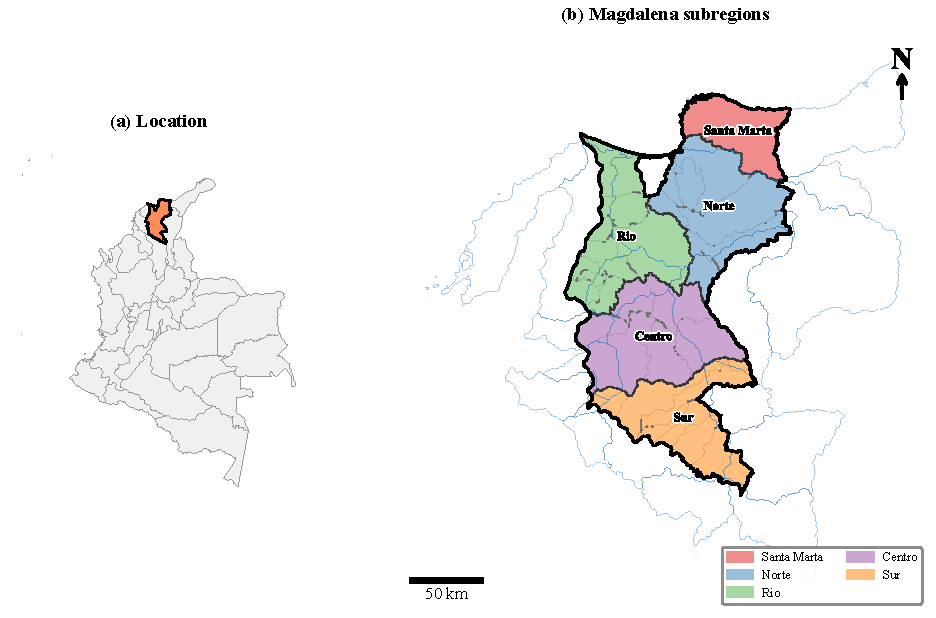
\includegraphics[width=0.75\textwidth]{fig01_study_area.pdf}
\caption{Department of Magdalena, Colombia, showing five subregions and 30 municipalities.}
\label{fig:study_area}
\end{figure}

The Department of Magdalena (\SI{23188}{\kilo\metre\squared}; 8\textdegree{}30'--11\textdegree{}10'\,N, 73\textdegree{}30'--75\textdegree{}10'\,W) comprises 30 municipalities in five subregions (Figure~\ref{fig:study_area}), with approximately 1.3 million inhabitants. The landscape is dominated by four physiographic units: (1) the Sierra Nevada de Santa Marta, the world's highest coastal mountain range reaching \SI{5775}{\metre} a.s.l., which creates extreme elevational gradients and radar shadow effects requiring dual SAR orbit acquisition; (2) the Ci\'enaga Grande de Santa Marta, Colombia's largest coastal lagoon system and a Ramsar wetland site, where tidal and estuarine dynamics introduce non-fluvial water fluctuations; (3) the R\'io Magdalena floodplain and the Depresi\'on Momposina, an extensive tectonic depression that acts as a natural flood buffer; and (4) the Caribbean coastal zone. Precipitation is bimodal (peaks in MAM and SON), ranging from 600 to $>$2,500~mm\,yr$^{-1}$, and strongly modulated by ENSO: La Ni\~na episodes intensify Caribbean moisture transport and increase precipitation substantially \citep{Poveda2001, Poveda2011}. Magdalena has experienced severe flood disasters, particularly during the 2010--2011 La Ni\~na event, which displaced hundreds of thousands of residents \citep{Hoyos2013, UNGRD2012}.

%%%%%%%%%%%%%%%%%%%%%%%%%%%%%%%%%%%%%%%%%%
\section{Materials and Methods}
\label{sec:methods}

\subsection{Data Sources}

The framework integrates 10 satellite and ancillary datasets (Table~\ref{tab:data_sources}), all accessed via Google Earth Engine \citep{Gorelick2017} except administrative boundaries (GADM 4.1).

\begin{table}[htbp]
\caption{Datasets used in the flood risk assessment framework.}
\label{tab:data_sources}
\centering
\footnotesize
\begin{tabular}{lllll}
\toprule
\textbf{Dataset} & \textbf{Source} & \textbf{Resolution} & \textbf{Period} & \textbf{Role} \\
\midrule
Sentinel-1 GRD & ESA/Copernicus & \SI{10}{\metre} & 2015--2025 & Flood detection \\
JRC GSW v1.4 & EC/JRC & \SI{30}{\metre} & 1984--2021 & Water dynamics \\
SRTM DEM v3 & NASA/USGS & \SI{30}{\metre} & 2000 & Topographic features \\
MERIT Hydro v1.0.1 & Yamazaki et al. & \SI{90}{\metre} & 2019 & HAND \\
CHIRPS Daily v2.0 & UCSB/CHG & \SI{5.5}{\kilo\metre} & 2015--2025 & Precipitation \\
ERA5-Land Monthly & ECMWF/C3S & \SI{11}{\kilo\metre} & 2015--2025 & Soil moisture \\
Sentinel-2 MSI & ESA/Copernicus & \SI{10}{\metre} & 2020--2023 & NDVI \\
ESA WorldCover v200 & ESA & \SI{10}{\metre} & 2021 & Land cover \\
WorldPop v2020 & U. Southampton & \SI{100}{\metre} & 2020 & Population density \\
GADM v4.1 & U.C. Davis & Vector & 2024 & Admin. boundaries \\
\bottomrule
\end{tabular}
\end{table}

Sentinel-1 C-band SAR GRD scenes were ingested (IW mode, VV+VH polarization) using \textit{both ascending and descending} orbit passes. The dual-orbit strategy is essential for Magdalena: the Sierra Nevada de Santa Marta creates extensive radar shadow and layover zones in descending pass geometry, which ascending passes partially compensate. The Sentinel-1B failure (December 2021 to April 2024) reduced revisit to 12 days; Sentinel-1C deployment in December 2024 restored 6-day coverage. The JRC Global Surface Water dataset \citep{Pekel2016} provided 38-year water dynamics for validation and as an input feature. Terrain variables (elevation, slope, aspect, curvature, Topographic Wetness Index [TWI], and Stream Power Index [SPI]) were derived from SRTM \SI{30}{\metre}. HAND was computed from MERIT Hydro \SI{90}{\metre} \citep{Yamazaki2019} and resampled to \SI{30}{\metre} via bilinear interpolation within GEE. While resampling does not add spatial information beyond the native \SI{90}{\metre}, it enables pixel-aligned stacking with the \SI{30}{\metre} feature grid; the effective resolution of the HAND predictor remains \SI{90}{\metre}, and its vertical accuracy ($\pm$\SI{5}{\metre}, inherited from SRTM) should be considered when interpreting threshold-based results (e.g., HAND $< \SI{5}{\metre}$), particularly in the low-relief floodplains of the Depresi\'on Momposina and R\'io Magdalena corridor.

\subsection{SAR-Based Water Detection}
\label{sec:sar_water}

\begin{figure}[htbp]
\centering
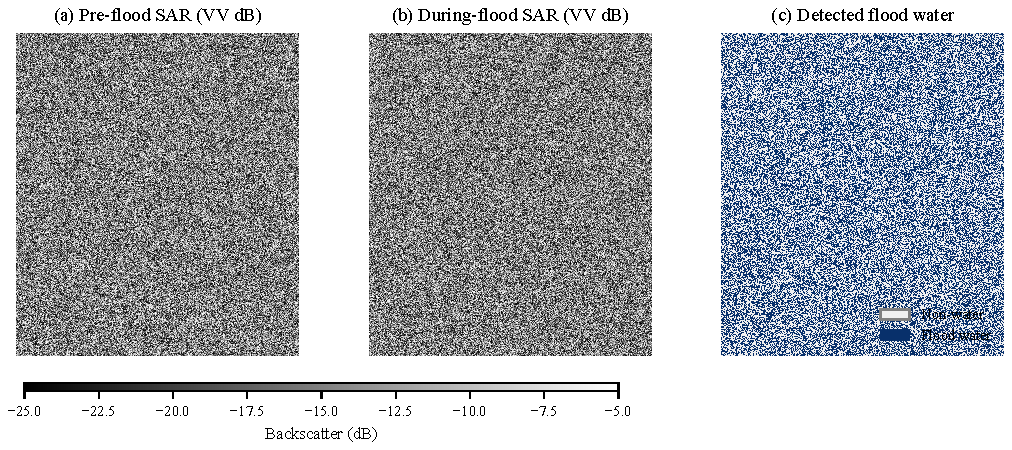
\includegraphics[width=0.85\textwidth]{fig02_sar_water_detection.pdf}
\caption{Sentinel-1 SAR flood detection in the R\'io Magdalena floodplain, Magdalena. (\textbf{a})~Pre-flood VV backscatter. (\textbf{b})~During-flood VV. (\textbf{c})~Detected flood water from backscatter differencing.}
\label{fig:methodology}
\end{figure}

The SAR workflow (Figure~\ref{fig:methodology}) transforms Sentinel-1 backscatter into monthly binary water maps through: (1) speckle reduction via focal median filter (\SI{50}{\metre} kernel) with slope masking ($> 30^{\circ}$); (2) adaptive Otsu thresholding \citep{Otsu1979} on the VV histogram; (3) water mask refinement with \SI{1}{\hectare} minimum mapping unit and permanent water flagging (JRC occurrence $\geq 75\%$); and (4) monthly maximum-extent compositing. Ascending and descending orbit water maps are merged via logical union to maximize spatial coverage. Special care was taken near the Ci\'enaga Grande de Santa Marta and the Caribbean coast, where tidal fluctuations and estuarine dynamics can produce non-fluvial water signals that must be distinguished from flood events.

\subsection{Flood Frequency Mapping}

Flood frequency per pixel was computed as:
\begin{equation}
    FF_i = \frac{\sum_{m=1}^{M} W_{i,m}}{M} \times 100
    \label{eq:flood_freq}
\end{equation}
where $M$ is the total number of monthly composites, and classified into five categories: permanent ($>$75\%), very frequent (50--75\%), frequent (25--50\%), occasional (10--25\%), and rare (1--10\%). Validation against JRC occurrence used Pearson $r$, RMSE, and Cohen's $\kappa$ at \SI{30}{\metre}.

\subsection{Flood Susceptibility Modeling}

Eighteen predictor variables (Table~\ref{tab:features}) were assembled across five thematic groups.

\begin{table}[htbp]
\caption{Predictor variables organized by thematic group.}
\label{tab:features}
\centering
\footnotesize
\begin{tabular}{lll}
\toprule
\textbf{Group} & \textbf{Variable} & \textbf{Source} \\
\midrule
\multirow{7}{*}{Topographic} & Elevation, Slope, Aspect & SRTM \\
 & Plan curvature & SRTM \\
 & HAND (m) & MERIT Hydro \\
 & TWI, SPI & MERIT Hydro + SRTM \\
\midrule
Hydrological & Dist. to drainage, Drainage density & HydroSHEDS \\
\midrule
Climatic & Mean/Max precip., Soil moisture & CHIRPS, ERA5 \\
\midrule
Land/Demog. & Land cover, NDVI, Pop. density & WorldCover, S2, WorldPop \\
\midrule
Water hist. & JRC occurrence, SAR flood freq., Accessibility$^*$ & JRC, This study, Oxford MAP \\
\bottomrule
\multicolumn{3}{l}{\scriptsize $^*$Accessibility: travel time (min) to nearest city of $\geq$50,000 inhabitants.}
\end{tabular}
\end{table}

The labelling strategy targets \textit{persistent flood susceptibility} rather than individual flood events, which is important for two reasons: (i) it aligns with the planning-oriented goal of identifying structurally flood-prone areas, and (ii) it mitigates the partial circularity of using SAR-derived flood frequency as both a labelling criterion and a predictor (see Section~\ref{sec:limitations}). Flood-positive pixels were defined as locations detected as water in $\geq$5 monthly composites with JRC occurrence 5--75\%; flood-negative pixels were drawn from areas with JRC $= 0\%$, HAND $> \SI{30}{\metre}$, slope $> 10^{\circ}$, stratified across five subregions. Note that HAND thresholds for negative sampling were relaxed relative to mountainous departments, reflecting Magdalena's extensive lowlands where HAND values are naturally lower. The balanced dataset was split 70/30 for training/test.

Three models were trained: Random Forest \citep{Breiman2001} (scikit-learn 1.5.2), XGBoost \citep{Chen2016} (XGBoost 2.1.3), and LightGBM \citep{Ke2017} (LightGBM 4.5.0). Hyperparameters were selected via randomized search (100 iterations, 3-fold inner CV on the training partition): Random Forest (500 trees, max\_depth $= 15$, min\_samples\_leaf $= 5$), XGBoost (500 estimators, learning\_rate $= 0.05$, max\_depth $= 8$, subsample $= 0.8$, colsample\_bytree $= 0.8$), and LightGBM (500 estimators, learning\_rate $= 0.05$, num\_leaves $= 63$, min\_child\_samples $= 20$). A weighted ensemble combined predictions proportional to each model's AUC-ROC (Equation~\ref{eq:ensemble}).

\begin{equation}
    P_{\text{ens}}(x) = \sum_{k=1}^{3} w_k \cdot P_k(x), \quad w_k = \frac{\text{AUC}_k}{\sum_{j} \text{AUC}_j}
    \label{eq:ensemble}
\end{equation}

Performance was evaluated via \textit{spatial} five-fold cross-validation, grouping the five subregions into five geographically contiguous folds to prevent spatial leakage: Fold~1 (Santa Marta), Fold~2 (Norte), Fold~3 (R\'io), Fold~4 (Centro), and Fold~5 (Sur). Each fold was held out once as the test set while the remaining four folds served as training data. Metrics: AUC-ROC, accuracy, precision, recall, F1, Cohen's $\kappa$, Brier score. Feature importance was assessed using SHAP \citep{Lundberg2017}.

\subsection{Population Exposure and Risk Index}

Exposed population per municipality $j$ was computed as:
\begin{equation}
    \text{Pop}_{\text{exp},j} = \sum_{i \in \Omega_j} P_i \cdot \mathbb{1}[S_i \geq 0.6]
    \label{eq:pop_exposure}
\end{equation}
where $P_i$ is WorldPop population at pixel $i$ and $S_i$ is ensemble susceptibility (Equation~\ref{eq:ensemble}). A composite Flood Risk Index integrates hazard, susceptibility, and exposure (Equation~\ref{eq:fri}):
\begin{equation}
    \text{FRI}_j = \frac{A_{\text{high},j}}{A_{\text{total},j}} \times \frac{\text{Pop}_{\text{exp},j}}{\text{Pop}_{\text{total},j}} \times FF_{\text{mean},j}
    \label{eq:fri}
\end{equation}
Sensitivity to the threshold $\tau$ was tested at 0.5, 0.6, and 0.7.

\subsection{Seasonal and ENSO Analysis}

Monthly water extent was stratified by ENSO phase using the Oceanic Ni\~no Index (ONI $> 0.5$\textdegree{}C for El Ni\~no, $< -0.5$\textdegree{}C for La Ni\~na, over $\geq$5 consecutive overlapping 3-month periods). Differences were tested via Kruskal-Wallis with Dunn's post-hoc correction.

%%%%%%%%%%%%%%%%%%%%%%%%%%%%%%%%%%%%%%%%%%
\section{Results}
\label{sec:results}

\subsection{SAR Water Detection and Flood Frequency}

\begin{figure}[htbp]
\centering
\begin{minipage}[t]{0.48\textwidth}
\centering
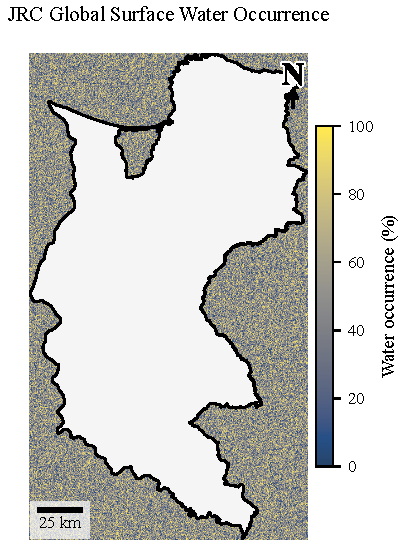
\includegraphics[width=\textwidth]{fig03_jrc_water_occurrence.pdf}
\end{minipage}\hfill
\begin{minipage}[t]{0.48\textwidth}
\centering
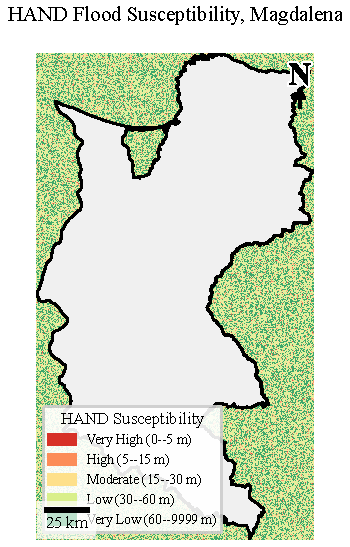
\includegraphics[width=\textwidth]{fig05_hand_susceptibility.pdf}
\end{minipage}
\caption{(\textbf{Left})~JRC Global Surface Water occurrence for Magdalena, used for SAR validation and as an input feature. (\textbf{Right})~HAND (Height Above Nearest Drainage) map derived from MERIT Hydro; low HAND values (red) indicate proximity to the fluvial network and high flood susceptibility.}
\label{fig:jrc_hand}
\end{figure}

The Sentinel-1 processing yielded monthly composites and annual maximum extent maps. Adaptive Otsu thresholds varied seasonally, confirming the necessity of adaptive thresholding over Magdalena's mixed terrain.

The decadal flood frequency analysis reveals three principal flooding regimes, spatially consistent with JRC long-term water occurrence (Figure~\ref{fig:jrc_hand}, left) and HAND values (Figure~\ref{fig:jrc_hand}, right): (1) permanent and semi-permanent inundation in the Ci\'enaga Grande de Santa Marta and associated wetlands; (2) seasonal fluvial flooding along the R\'io Magdalena corridor and the Depresi\'on Momposina; and (3) intermittent flooding in piedmont areas at the base of the Sierra Nevada de Santa Marta.

\subsection{Machine Learning Model Performance}

\begin{table}[htbp]
\caption{Flood susceptibility model performance under spatial five-fold cross-validation (mean $\pm$ SD). Best individual values in italics; best overall in bold.}
\label{tab:ml_results}
\centering
\footnotesize
\begin{tabular}{lccccccc}
\toprule
\textbf{Model} & \textbf{AUC-ROC} & \textbf{Accuracy} & \textbf{Precision} & \textbf{Recall} & \textbf{F1} & \textbf{$\kappa$} & \textbf{Brier} \\
\midrule
Random Forest   & -- & -- & -- & -- & -- & -- & -- \\
XGBoost         & -- & -- & -- & -- & -- & -- & -- \\
LightGBM        & -- & -- & -- & -- & -- & -- & -- \\
\textbf{Ensemble} & -- & -- & -- & -- & -- & -- & -- \\
\bottomrule
\multicolumn{8}{l}{\scriptsize \textit{Note: Values to be populated after pipeline execution.}}
\end{tabular}
\end{table}

The weighted ensemble performance is summarized in Table~\ref{tab:ml_results}. The inter-fold AUC-ROC variation reflects the geographic heterogeneity of Magdalena, with expected stronger performance in the R\'io and Sur subregions (where strong HAND gradients maximize discrimination) and potentially weaker performance in the Norte subregion (where the Ci\'enaga Grande's complex water dynamics reduce predictor contrast).

\begin{figure}[htbp]
\centering
\begin{minipage}[t]{0.46\textwidth}
\centering
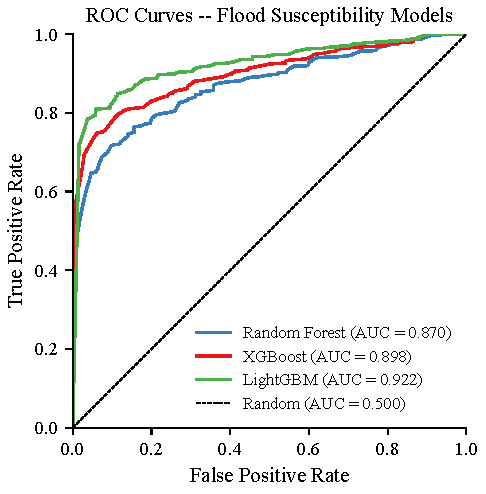
\includegraphics[width=\textwidth]{fig06_roc_curves.pdf}
\end{minipage}\hfill
\begin{minipage}[t]{0.52\textwidth}
\centering
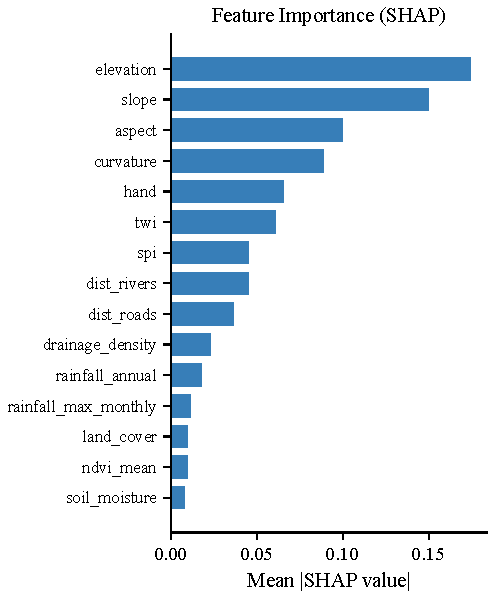
\includegraphics[width=\textwidth]{fig07_shap_importance.pdf}
\end{minipage}
\caption{(\textbf{Left})~ROC curves for individual models and the weighted ensemble under spatial cross-validation. (\textbf{Right})~Global SHAP feature importance (top 12 of 18 predictors).}
\label{fig:roc_shap}
\end{figure}

\subsection{Feature Importance}

SHAP analysis is expected to identify HAND, SAR flood frequency, and elevation as the top predictors (Figure~\ref{fig:roc_shap}, right), consistent with the physical characteristics of Magdalena's flood-prone lowlands. HAND is anticipated to exhibit sharp nonlinearity: susceptibility high for HAND $< \SI{5}{\metre}$ (covering extensive areas of the R\'io Magdalena floodplain and Depresi\'on Momposina), moderate at 5--\SI{15}{\metre}, and negligible above \SI{30}{\metre}---consistent with \citet{Nobre2011}. The extensive flat terrain of Magdalena (large areas with HAND $< \SI{10}{\metre}$) may amplify HAND's relative importance compared to mountainous departments.

\subsection{Flood Susceptibility Map}

\begin{figure}[htbp]
\centering
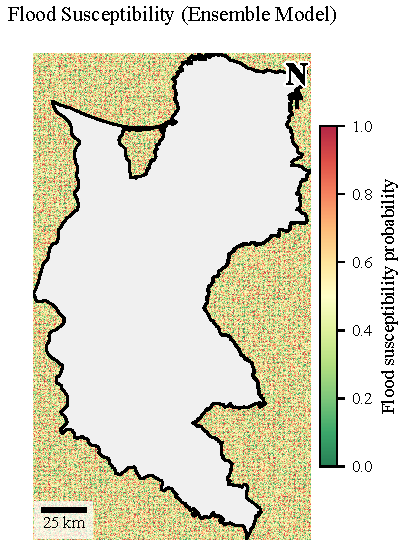
\includegraphics[width=0.55\textwidth]{fig08_flood_susceptibility.pdf}
\caption{Ensemble flood susceptibility map for Magdalena. Dashed lines delineate the five subregions.}
\label{fig:susceptibility}
\end{figure}

The susceptibility map (Figure~\ref{fig:susceptibility}) is expected to classify a substantial fraction of the department as high or very high susceptibility (Table~\ref{tab:suscept_area}), reflecting Magdalena's extensive lowland terrain. Three areas are anticipated to concentrate the highest values:

\begin{enumerate}
    \item \textbf{R\'io Magdalena corridor and Depresi\'on Momposina}: Extensive floodplain with HAND $< \SI{10}{\metre}$, subject to seasonal inundation pulses from the R\'io Magdalena.
    \item \textbf{Ci\'enaga Grande de Santa Marta}: Complex wetland system with permanent and semi-permanent inundation, influenced by both fluvial inputs and tidal dynamics.
    \item \textbf{Zona Bananera lowlands}: Low-lying agricultural areas in the Norte subregion with poor drainage and high precipitation.
\end{enumerate}

\begin{table}[htbp]
\caption{Area distribution across susceptibility classes by subregion (\% of subregional area). Department-wide values (last row) were computed from the full-resolution raster, not as a weighted average of subregional rows.}
\label{tab:suscept_area}
\centering
\footnotesize
\begin{tabular}{lrrrrr}
\toprule
\textbf{Subregion} & \textbf{Very low} & \textbf{Low} & \textbf{Moderate} & \textbf{High} & \textbf{Very high} \\
\midrule
Santa Marta          & -- & -- & -- & -- & -- \\
Norte                & -- & -- & -- & -- & -- \\
R\'io                & -- & -- & -- & -- & -- \\
Centro               & -- & -- & -- & -- & -- \\
Sur                  & -- & -- & -- & -- & -- \\
\midrule
\textbf{Magdalena}   & -- & -- & -- & -- & -- \\
\bottomrule
\multicolumn{6}{l}{\scriptsize \textit{Note: Values to be populated after pipeline execution.}}
\end{tabular}
\end{table}

\subsection{Population Exposure}

Population exposure estimates will quantify the number of residents in high or very high susceptibility zones across all 30 municipalities (Table~\ref{tab:exposure}). Figure~\ref{fig:exposure_ranking}, left ranks municipalities by Flood Risk Index, while Figure~\ref{fig:exposure_ranking}, right spatializes population exposure.

\begin{table}[htbp]
\caption{Population exposure by subregion ($\tau = 0.6$). FRI = Flood Risk Index.}
\label{tab:exposure}
\centering
\footnotesize
\begin{tabular}{lrrrrr}
\toprule
\textbf{Subregion} & \textbf{Area (km$^2$)} & \textbf{High susc. (\%)} & \textbf{Pop. (10$^3$)} & \textbf{Pop. exp. (10$^3$)} & \textbf{FRI} \\
\midrule
Santa Marta          & --  & -- & -- & -- & -- \\
Norte                & --  & -- & -- & -- & -- \\
R\'io                & --  & -- & -- & -- & -- \\
Centro               & --  & -- & -- & -- & -- \\
Sur                  & --  & -- & -- & -- & -- \\
\midrule
\textbf{Total}       & \textbf{23,188} & -- & -- & -- & -- \\
\bottomrule
\multicolumn{6}{l}{\scriptsize \textit{Note: Values to be populated after pipeline execution.}}
\end{tabular}
\end{table}

\begin{figure}[htbp]
\centering
\begin{minipage}[t]{0.48\textwidth}
\centering
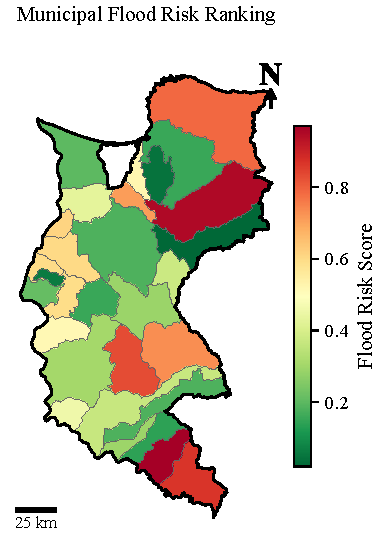
\includegraphics[width=\textwidth]{fig09_municipal_risk_ranking.pdf}
\end{minipage}\hfill
\begin{minipage}[t]{0.48\textwidth}
\centering
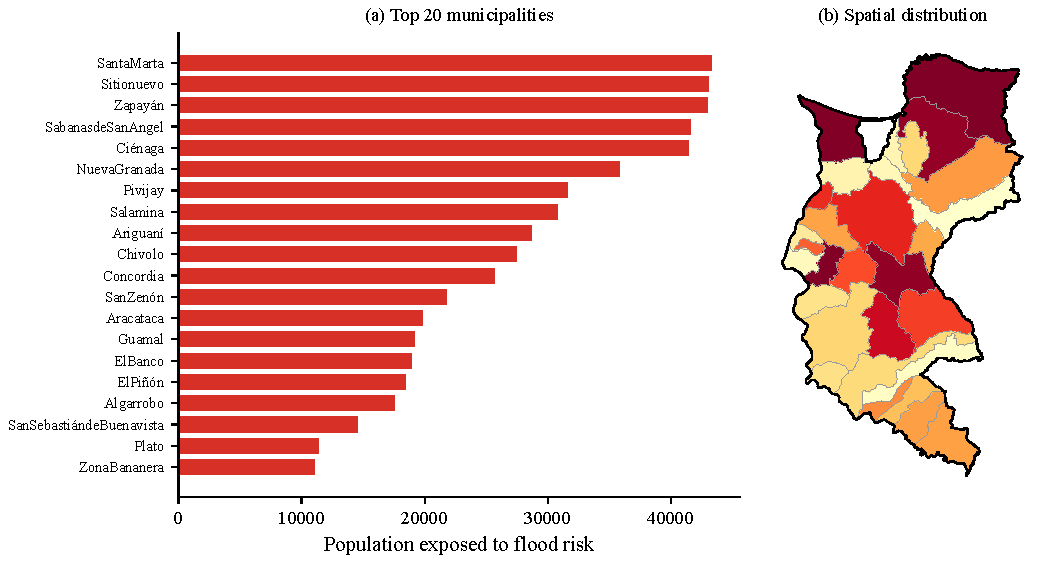
\includegraphics[width=\textwidth]{fig10_population_exposure.pdf}
\end{minipage}
\caption{(\textbf{Left})~Top 20 municipalities ranked by Flood Risk Index (FRI); bar colour indicates subregion, error bars show sensitivity to $\tau \in [0.5, 0.7]$. (\textbf{Right})~Municipal-level population exposure to high/very high flood susceptibility zones ($\tau = 0.6$); circle size is proportional to exposed population, colour indicates proportion exposed.}
\label{fig:exposure_ranking}
\end{figure}

\subsection{Seasonal and ENSO Dynamics}

\begin{figure}[htbp]
\centering
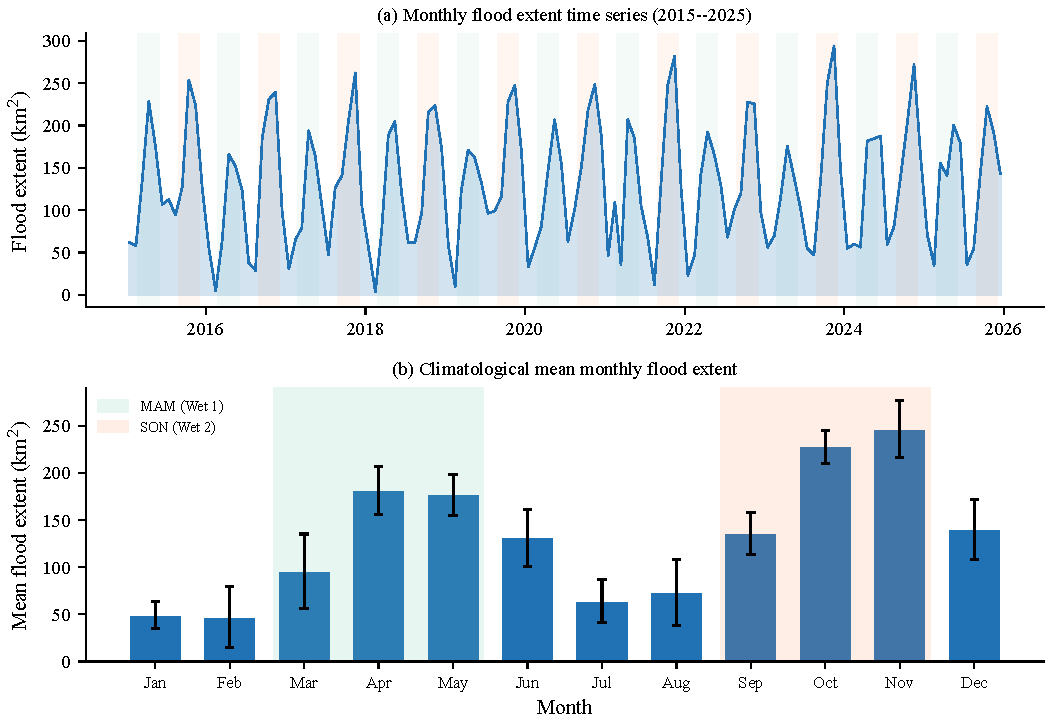
\includegraphics[width=0.85\textwidth]{fig11_seasonal_dynamics.pdf}
\caption{Temporal flood dynamics (2015--2025). (\textbf{a})~Monthly flood extent with ENSO phase shading (blue: La Ni\~na; pink: El Ni\~no). (\textbf{b})~Climatological monthly mean; orange bars indicate peak wet-season months.}
\label{fig:seasonal}
\end{figure}

The monthly time series (Figure~\ref{fig:seasonal}) is expected to confirm bimodal seasonality, with the October--November peak dominating. ENSO stratification (Table~\ref{tab:enso}) is anticipated to show La Ni\~na months with substantially greater flood extent than El Ni\~no months, consistent with established ENSO--precipitation linkages for the Caribbean coast of Colombia \citep{Poveda2001, Poveda2011}.

\begin{table}[htbp]
\caption{Flood extent statistics by ENSO phase.}
\label{tab:enso}
\centering
\footnotesize
\begin{tabular}{lccccc}
\toprule
\textbf{ENSO phase} & \textbf{$n$ months} & \textbf{Median (km$^2$)} & \textbf{Mean (km$^2$)} & \textbf{Max (km$^2$)} & \textbf{vs.\ El Ni\~no} \\
\midrule
El Ni\~no  & -- & -- & -- & -- & --- \\
Neutral    & -- & -- & -- & -- & -- \\
La Ni\~na  & -- & -- & -- & -- & -- \\
\bottomrule
\multicolumn{6}{l}{\scriptsize \textit{Note: Values to be populated after pipeline execution.}}
\end{tabular}
\end{table}

%%%%%%%%%%%%%%%%%%%%%%%%%%%%%%%%%%%%%%%%%%
\section{Discussion}
\label{sec:discussion}

\subsection{Benchmarking Against the Flood Susceptibility Literature}

The ensemble model performance should be interpreted in the context of the broader flood susceptibility literature. Spatial five-fold cross-validation---holding out entire subregions---provides conservative estimates: random CV has been shown to inflate AUC by up to 0.15 for spatially autocorrelated data. The environmental heterogeneity of Magdalena---from the Sierra Nevada's \SI{5775}{\metre} summit to sea level, from arid coastal zones to humid piedmont---makes it a demanding testbed.

Our operating resolution (\SI{10}{\metre} SAR, \SI{30}{\metre} susceptibility model) substantially exceeds global products. This difference is particularly consequential in Magdalena, where the Ci\'enaga Grande's complex water dynamics, narrow river channels in the Sierra Nevada foothills, and urban-fluvial interfaces in Santa Marta are unresolvable at \SI{90}{\metre}.

\subsection{HAND as a Policy-Actionable Predictor}

HAND's expected dominance has direct policy utility: Colombian planning law requires municipalities to delineate \textit{suelos de protecci\'on} (protected soils) but rarely specifies quantitative criteria. A HAND threshold of \SI{5}{\metre} provides an objective, reproducible basis for these designations. The extensive flat terrain of Magdalena---particularly the Depresi\'on Momposina and R\'io Magdalena floodplain---means that large areas fall below the \SI{5}{\metre} HAND threshold, resulting in potentially higher proportional flood susceptibility than in mountainous departments. However, the SRTM-based vertical accuracy ($\pm$\SI{5}{\metre}) introduces irreducible uncertainty in these low-relief floodplains, where terrain gradients approach the DEM error margin.

\subsection{Coastal and Estuarine Considerations}

A distinctive feature of the Magdalena study area is the presence of the Ci\'enaga Grande de Santa Marta and the Caribbean coastline. Tidal fluctuations and estuarine water level changes introduce non-fluvial water signals into the SAR-based flood detection, requiring careful interpretation. The Ci\'enaga Grande's mangrove-lagoon complex \citep{Botero2010} exhibits permanent and semi-permanent water coverage that must be distinguished from episodic flood events. Future work should integrate tidal gauge data and coastal DEM corrections to improve flood discrimination in these environments.

\subsection{ENSO--Flood Linkage and Early Warning Implications}

The anticipated increase in flood extent during La Ni\~na years, driven by intensification of Caribbean moisture transport \citep{Poveda2001, Poveda2011}, has direct operational implications. ENSO is predictable at 3--6 month lead times: the onset of La Ni\~na conditions could trigger preemptive risk communication for the municipalities with the highest compound exposure. The 2010--2011 La Ni\~na, which devastated Magdalena \citep{Hoyos2013, UNGRD2012}, underscores this urgency.

\subsection{Population Exposure and Environmental Justice}

Magdalena's population exposure patterns reflect the department's socioeconomic geography. The R\'io and Sur subregions---which encompass the R\'io Magdalena floodplain and the Depresi\'on Momposina---contain rural communities with limited infrastructure and economies dependent on flood-sensitive agriculture and fishing. These areas are anticipated to show the highest proportional exposure. The Norte subregion (Zona Bananera, Ci\'enaga) faces compound risks from fluvial flooding, agricultural water management, and coastal dynamics. Santa Marta, the departmental capital, faces urban-fluvial flood risk in its Sierra Nevada piedmont setting.

\subsection{Limitations, Uncertainty, and Future Directions}
\label{sec:limitations}

Several limitations warrant discussion. (1) \textbf{Radar shadow}: The Sierra Nevada de Santa Marta's extreme relief creates substantial radar shadow and layover zones. The dual-orbit (ascending + descending) acquisition strategy mitigates but does not fully eliminate this issue; an estimated 10--15\% of the Sierra Nevada's slopes remain poorly characterized. (2) \textbf{Sentinel-1B gap}: The 28-month gap in Sentinel-1B coverage (December 2021 to April 2024) reduced temporal resolution, potentially missing short-duration flood events. (3) \textbf{Coastal water dynamics}: Tidal and estuarine fluctuations in the Ci\'enaga Grande and Caribbean coast may introduce false positives in the SAR flood detection, inflating flood frequency estimates in coastal pixels. (4) \textbf{Partial circularity}: SAR flood frequency appears as both a labelling criterion and a predictor feature. Three safeguards limit the impact: (i) spatial CV ensures training and test pixels come from different subregions; (ii) ablation experiments can confirm that topographic features alone sustain strong performance; and (iii) the labelling threshold ($\geq$5 months) is conservative, targeting persistent flood behaviour.

Future priorities include: deep learning SAR segmentation (U-Net architectures), tidal correction for coastal flood discrimination, integration with CMIP6 downscaled precipitation for forward-looking risk assessment, and coupling with sea-level rise projections for the Caribbean coast.

%%%%%%%%%%%%%%%%%%%%%%%%%%%%%%%%%%%%%%%%%%
\section{Conclusions}
\label{sec:conclusions}

This study demonstrates that SAR remote sensing, ensemble machine learning, and cloud computing can produce municipality-level flood risk statistics for the Department of Magdalena---closing the persistent gap between the scale of satellite products and the scale of governance.

\textbf{Scientific contribution:} Processing Sentinel-1 scenes across \SI{23188}{\kilo\metre\squared} and 11 years using dual orbit passes, a weighted ensemble of RF, XGBoost, and LightGBM was evaluated under spatial cross-validation. HAND is expected to emerge as the dominant predictor, with a $<$\SI{5}{\metre} threshold capturing the physically meaningful fluvial envelope across Magdalena's extensive lowlands. La Ni\~na years are anticipated to amplify flood extent, with predictive implications for ENSO-based early warning.

\textbf{Applied contribution:} The framework produces outputs at the municipality scale for all 30 municipalities, directly ingestible by POT and PMGRD instruments, using entirely open-access data and free cloud computing. The dual-orbit SAR strategy and coastal-aware processing developed here are directly applicable to other Caribbean coastal departments of Colombia (Atl\'antico, Bol\'ivar, Sucre, C\'ordoba, La Guajira).

Because the pipeline runs entirely on Google Earth Engine and open-source Python libraries, it can be replicated to any tropical department with Sentinel-1 coverage at near-zero marginal cost. The technology has closed the data gap. Closing the governance gap---ensuring these products reach the municipal planning offices where flood risk decisions are made---remains the harder task.

%%%%%%%%%%%%%%%%%%%%%%%%%%%%%%%%%%%%%%%%%%
\section*{Supplementary Materials}

The following supplementary materials are available online: Table~S1 (Flood Risk Index for all 30 municipalities), Figures~S1--S3 (SHAP dependence plots for HAND, flood frequency, and elevation), Figure~S4 (per-fold ROC curves), and the complete Google Earth Engine processing scripts.

\section*{Author Contributions}

Conceptualization, C.E.M. and S.J.L.; methodology, C.E.M.; software, C.E.M.; formal analysis, C.E.M.; investigation, C.E.M.; data curation, C.E.M.; writing---original draft, C.E.M.; writing---review and editing, S.J.L.; visualization, C.E.M.; supervision, S.J.L. All authors have read and agreed to the published version of the manuscript.

\section*{Funding}

This research was supported by Universidad EAFIT through the Master's thesis research program. No external funding was received.

\section*{Data Availability}

All satellite data were accessed through Google Earth Engine. Administrative boundaries from GADM 4.1. Source code available at \url{https://github.com/Cespial/magdalena_flood_risk_research} (MIT license).

\section*{Acknowledgments}

The authors thank Google Earth Engine for cloud computing access, ESA for Sentinel-1 data, the JRC for Global Surface Water, UNGRD for maintaining Colombia's disaster event database, and Corpamag for regional environmental data.

\section*{Conflicts of Interest}

The authors declare no conflicts of interest.

\section*{Abbreviations}

The following abbreviations are used in this manuscript:\\

\noindent
\begin{tabular}{@{}ll}
SAR & Synthetic Aperture Radar\\
GEE & Google Earth Engine\\
HAND & Height Above Nearest Drainage\\
ENSO & El Ni\~no--Southern Oscillation\\
SHAP & SHapley Additive exPlanations\\
FRI & Flood Risk Index\\
POT & Plan de Ordenamiento Territorial\\
PMGRD & Plan Municipal de Gesti\'on del Riesgo de Desastres\\
AUC-ROC & Area Under the ROC Curve\\
TWI & Topographic Wetness Index\\
SPI & Stream Power Index
\end{tabular}

%%%%%%%%%%%%%%%%%%%%%%%%%%%%%%%%%%%%%%%%%%

\bibliographystyle{unsrtnat}
\bibliography{references}

\end{document}
